\documentclass[]{beamer}
\usepackage[utf8]{inputenc}
\usepackage{polski}
\usepackage[polish]{babel}

\usepackage{amsmath}
\usepackage{esint}
\usepackage{graphicx}

\title[Co kryje PNG?]{Co kryje PNG?}
\author[Krzysztof Kwapisiewicz]{Krzysztof Kwapisiewicz}
\institute{Software Engineer @ Codilime}
\date{02.09.2016}

\AtBeginSection[]
{
  \begin{frame}
    \tableofcontents[currentsection]
  \end{frame}
}

\AtBeginSubsection[]
{
  \begin{frame}
    \tableofcontents[currentsection,currentsubsection]
  \end{frame}
}

\begin{document}
\begin{frame}
  \begin{titlepage}
  \end{titlepage}
\end{frame}

\section[Co to ten PNG?]{Co to ten PNG?}
\begin{frame}{Co mówi wiki?}
  \begin{itemize}
    \item Rastrowy format plików graficznych oraz system bezstratnej kompresji danych graficznych
    \item Obsługuje stopniowaną przezroczystość (tzw.\ kanał alfa)
    \item Umożliwia zarządzanie kolorami (paleta kolorów, przestrzeń barw etc.)
    \item Pozwala na przechowywanie metadanych
  \end{itemize}
  \begin{center}
    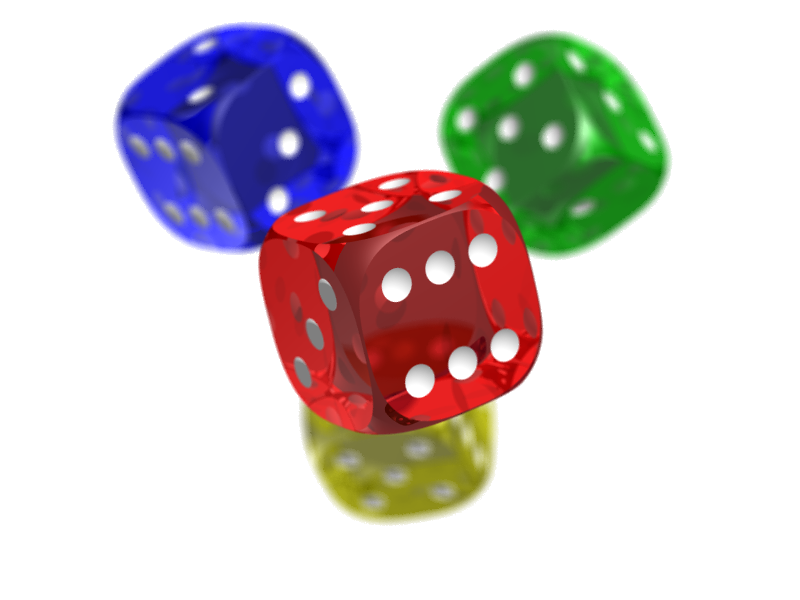
\includegraphics[width=0.5\textwidth]{../img/example.png}
  \end{center}
\end{frame}

\begin{frame}{Co mówi dokumentacja?}
  \begin{center}
    \begin{tabular}{|c|c|c|c|}
      \hline
      \textbf{Długość} & \textbf{Rodzaj} & \textbf{Dane} & \textbf{CRC} \\
      \hline
      4 bajty & 4 bajty & \textit{Długość} bajtów & 4 bajty \\
      \hline
    \end{tabular}
  \end{center}
\end{frame}

\begin{frame}
  Krytyczne chunki:
  \begin{itemize}
    \item \textbf{IHDR} - pierwszy chunk, zawiera podstawowe info o obrazie jak wysokość i szerokość
    \item \textbf{PLTE} - paleta (lista) kolorów
    \item \textbf{IDAT} - ,,mięso'' obrazu
    \item \textbf{IEND} - koniec pliku
  \end{itemize}

  Pomocnicze chunki: bKGD, cHRM, gAMA, hIST, iCCP, iTXt, pHYs, sBIT, sPLT, sRGB, sTER, tEXt, tIME, tRNS, zTXt
\end{frame}

\end{document}
